\documentclass[../../Report.tex]{subfiles}
\usepackage[italian]{babel}

\begin{document}
\chapter{Implementazione}
\section{Data Preprocessing}
La fase di preprocessing dei dati consiste nel preparare i dati per l'addestramento del modello.
Una volta acqusiti i dati e averne studiato le peculiarità e le caratteristiche, si procede con la pulizia dei dati.
Abbiamo usato il metodo \textit{pivot\_table} di Pandas per creare una tabella pivot che contiene i genome-score degli utenti per ogni film che lo possiede (andando così a ridurre la cardialità da 60k a 13.816).\\
In seguito a ciò verrà effettuata una merge con un i generi dei film.
Ci siamo inoltre andati a focalizzare sui voti da parte degli utenti, raggruppandoli per film ci abbiamo calcolato la media dei voti.
Quest'ultimo sarà il nostro \textit{target} per l'addestramento del modello.\\

\section{Modeling}
La nostra fase di modellazione include uno studio di regressione basato sulla predizione del voto medio di un film dati i suoi genome-score.
Abbiamo inoltre applicato una tecnica di \textit{PCA} con l'obiettivo di ridurre la cardinalità dei dati, eseguendo l'addestramento sia con che senza la PCA su tutti i modelli al fine di confrontarne i risultati.

Eseguiamo il train-test split con un rapporto 80-20 ed in seguito addestreremo il nostro modello.
\subsection{Tecniche di ML Supervisionate con Approccio non-Deep}
In questa sezione verranno descritte le tecniche di ML supervisionate con approccio non-Deep utilizzate per la predizione del voto medio di un film.
\begin{itemize}
    \item \textbf{Linear Regression}: La regressione lineare è una tecnica di ML supervisionata che permette di predire il valore di una variabile dipendente a partire da una o più variabili indipendenti.
    \begin{itemize}
        \item \textbf{Ridge}: Ridge è un algoritmo di regressione lineare che utilizza un termine di regolarizzazione per eviare problemi di multicollinearità. Il parametro di regolarizzazione controlla l'importanza del termine di regolarizzazione nella funzione di costo
        \item \textbf{Lasso}: Lasso è un algoritmo di ML supervisionato che permette di effettuare la regressione di un dato mediante la creazione di un modello lineare.
    \end{itemize}
    \item \textbf{Deicision Tree}: Decision Tree è un algoritmo di ML supervisionato che permette di effettuare la classificazione o la regressione di un dato mediante la creazione di un albero di decisione.
    \item \textbf{Random Forest}: Random Forest è un algoritmo di ML supervisionato che permette di effettuare la classificazione o la regressione di un dato mediante la creazione di più alberi (Metodo di Emsable Learning).
    \item \textbf{SVR}: Support Vector Regression è un algoritmo che cerca di trovare una funzione che minimizzi la distanza tra i dati di training e una fascia di tolleranza definita dall'utente.
    \item \textbf{KNN}: K-Nearest Neighbors è un algoritmo di ML supervisionato che permette di effettuare la classificazione o la regressione di un dato cerca di stimare il valore di una variabile dipendente su nuovi dati in base alla loro vicinanza ad altri dati di training.
\end{itemize}

Per ogni modello precedentemente citato è stato applicato il Tuning dei parametri per cercare di ottimizzare il modello.
Attraverso la funzione \textit{GridSearch} di Scikit-Learn abbiamo cercato di trovare i migliori parametri per ogni modello.

\subsubsection{Tuning dei Parametri}
Per ogni modello precedentemente citato è stato applicato il Tuning dei parametri per cercare di ottimizzare il modello.
Attraverso la funzione \textit{GridSearch} di Scikit-Learn abbiamo cercato di trovare i migliori parametri per ogni modello, come nel seguente esempio:
\begin{lstlisting}[language=Python]
    def tuning(self):
        search = GridSearchCV(estimator = self.svr, param_grid= self.params, cv = 3, n_jobs = 6)
        search.fit(self.X_train_t, self.y_train)
        print(search.best_params_)
        print(search.best_score_)
        self.svr = search.best_estimator_
\end{lstlisting}
\subsection{Linear Regression}
Il modello di Linear Regression ci permette di operare una regressione lineare tra i nostri dati(una regressione multivariable).
In questo specifico modello non abbiamo particolari parametri per cui fare tuning.
Di conseguenza andremo a vedere i risultati del tuning per i modelli che usano la regressione lineare: Lasso e Ridge
\subsubsection{Ridge}
Ridge è un algoritmo di ML supervisionato che permette di effettuare la regressione di un dato mediante la creazione di un modello lineare.
Si basa su un valore di regolarizzazione che permette di evitare problemi di multicollinearità.
Per cercare il valore $\alpha$ apposito abbiamo utilizzato la funzione \textit{RidgeCV} di Scikit-Learn, che permette di trovare il valore ottimale di $\alpha$, ed effettuare la Cross Validation.

\begin{table}[h]
    \centering
    \begin{tabular}{|c|c|c|}
    \hline
\textbf{Modello} & \textbf{senza PCA} & \textbf{PCA} \\ \hline
\textbf{$\alpha$} & 6.0 & 2.5\\ \hline
\end{tabular}
\end{table}


\subsubsection{Lasso}
Lasso è un algoritmo di ML supervisionato che permette di effettuare la regressione di un dato mediante la creazione di un modello lineare.
Abbiamo cercato anche qui di ottimizzare il valore $\alpha$ abbiamo utilizzato la funzione \textit{LassoCV} di Scikit-Learn, che permette di trovare il valore ottimale di $\alpha$, ed effettuare la Cross Validation.


\begin{table}[h]
    \centering
    \begin{tabular}{|c|c|c|}
    \hline
\textbf{Modello} & \textbf{senza PCA} & \textbf{PCA} \\ \hline
\textbf{Alpha} &  7.425262873115622e-05 &   0.0005675190692206821 \\ \hline
\end{tabular}
\end{table}
\subsection{Decision Tree}
Decision Tree è un algoritmo di ML supervisionato che permette di effettuare la regressione di un dato mediante la creazione di un albero di decisione.
Abbiamo avuto bisogno di fare il tuning di piu parametri, in particolare:
\begin{lstlisting}[language=Python]
    self.params = {
                'splitter' : ['best','random'],
                'max_depth' : [None, 20,50,100],
                'min_samples_split' : [10, 50, 100, 200],
                'min_samples_leaf' : [2, 5, 10, 20],
                'max_features' : ['auto', 'sqrt', 'log2'],
                'max_leaf_nodes' : [None, 5, 10, 20],
    }
\end{lstlisting}
Abbiamo utilizzato la funzione \textit{GridSearchCV} di Scikit-Learn per trovare i migliori parametri per il modello, utilizzando un CV di 3 volendo mantenere coerenza con altre ricerche che con una CV maggiore avrebbero portato ad un incremento considerevole del tempo.
Di seguito i risultati ottenuti:\\
\begin{table}[H]
    \centering
    \begin{tabular}{|c|c|c|}
    \hline
    \textbf{Parametri} & \textbf{senza PCA} & \textbf{PCA} \\ \hline
    \textbf{max\_depth}& None & None\\
    \textbf{max\_features}& 'auto' &  'auto' \\
    \textbf{max\_leaf\_nodes}& None & None\\
    \textbf{min\_samples\_leaf}& 20 & 20\\
    \textbf{min\_samples\_split}& 50 & 100\\
    \textbf{splitter}& 'best' &  'best'\\
    \hline
\end{tabular}
\end{table}
Mostriamo inoltre il grafico che mostra l'andamento del Mean Test Score in funzione dei parametri, ricordando che nei modelli successivi verrá mostrato il grafico solo con dati senza PCA:
\begin{figure}[H]
    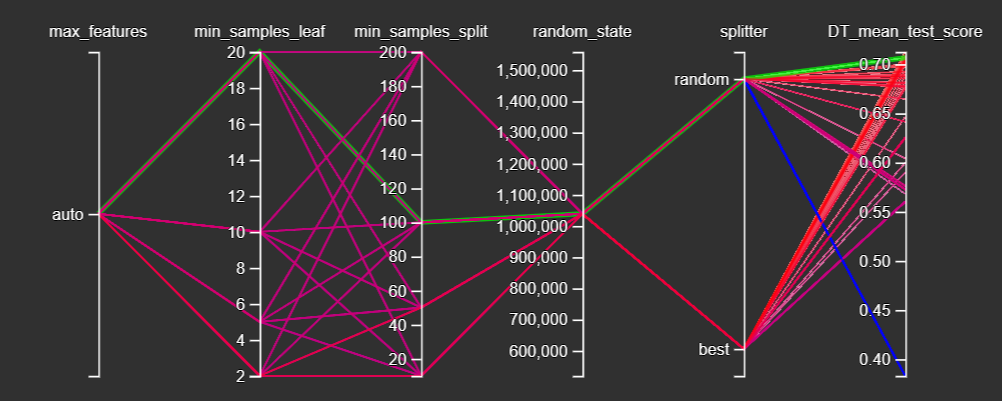
\includegraphics[width=.9\textwidth]{hpDT.png}
    \centering
\end{figure}
\subsection{Random Forest}
Random Forest è un algoritmo di ML supervisionato che permette di effettuare la regressione di un dato mediante la creazione di più alberi (Metodo di Emsable Learning).
I parametri su cui effettueremo il tuning sono:
\begin{lstlisting}[language=Python]
    self.params = {
        'n_estimators': [50,100,500],
        'max_depth': [None ,10, 50, 100],
        'min_samples_split': [2, 5, 10],
        'min_samples_leaf': [1, 2, 5],
        'max_features': ['auto', 'sqrt', 'log2'],
    }
\end{lstlisting}
Ottendendo i seguenti risultati:
\begin{table}[H]
    \centering
    \begin{tabular}{|c|c|c|}
    \hline
    \textbf{Parametri} & \textbf{senza PCA} & \textbf{PCA} \\ \hline
    \textbf{max\_depth}& None & None\\
    \textbf{max\_features}& 'auto' &  'auto' \\
    \textbf{min\_samples\_leaf}& 1 & 1\\
    \textbf{min\_samples\_split}& 2 & 2\\
    \textbf{n\_estimators}& 500 & 500\\
\hline

\end{tabular}
\end{table}
Qui di seguito inoltre riportiamo un grafico che mostra la distribuzione dei parametri e del Mean Test Score ottenuto:
\begin{figure}[H]
    \centering
    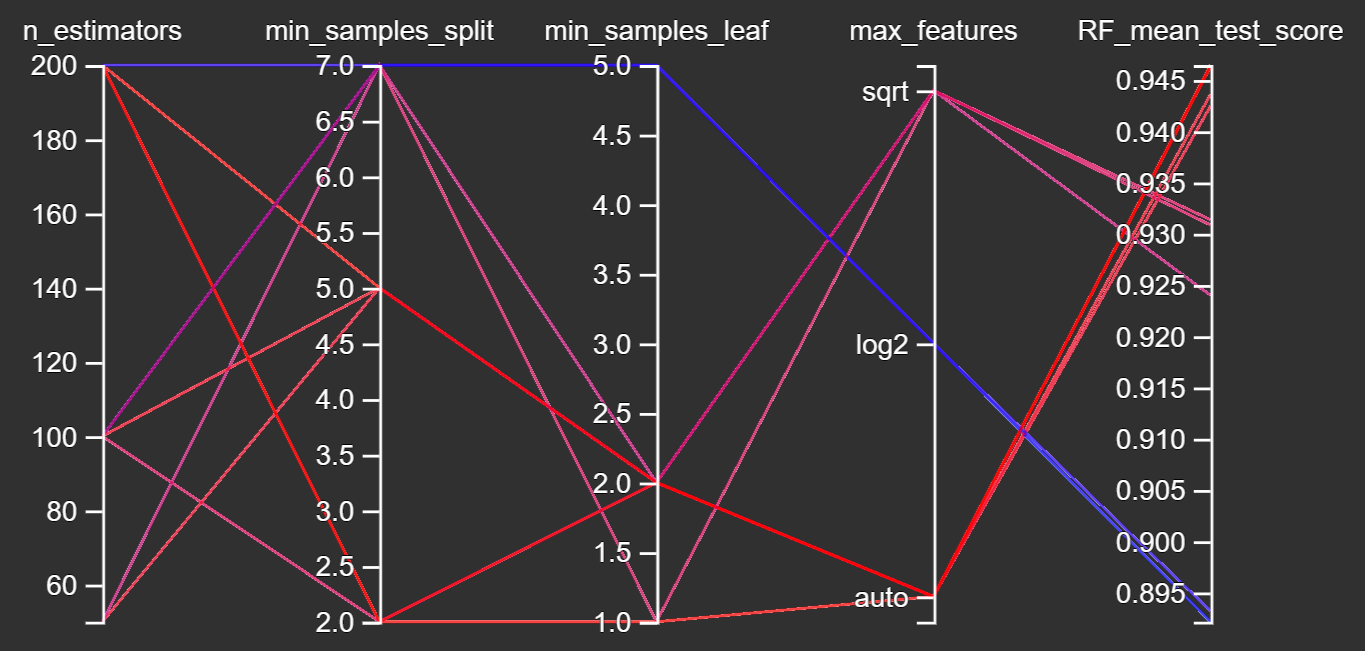
\includegraphics[width=.9\textwidth]{HP_RF.png}
\end{figure}

\subsection{SVR}
SVR è un algoritmo di ML supervisionato che permette di effettuare la regressione di un dato mediante la creazione di un modello lineare.
Due parametri rilvanti sono C e $\epsilon$: C è il parametro di regolarizzazione, mentre $\epsilon$ è il parametro che permette di definire la tolleranza per il modello.
\begin{lstlisting}[language=Python]
    self.params = {
        'kernel': ['linear','poly', 'rbf', 'sigmoid'],
        'C': [0.01, 0.1, 1, 10, 100],
        'gamma': [0.001, 0.01, 0.1, 1, 10],
        'epsilon': [0.01, 0.1, 1, 10]
    }
\end{lstlisting}
Ottendendo i seguenti risultati:
\begin{table}[H]
    \centering
    \begin{tabular}{|c|c|c|}
    \hline
    \textbf{Parametri} & \textbf{senza PCA} & \textbf{PCA} \\ \hline
    \textbf{C}& 1 & 100\\
    \textbf{epsilon}& 0.01 &  0.01 \\
    \textbf{gamma}& 0.01 & 0.001\\
    \textbf{kernel}& 'rbf' &  'rbf'\\
    \hline
\end{tabular}
\end{table}
Come per il modello precedente riportiamo il grafico dell'andamento dei parametri e del Mean Test Score:
\begin{figure}[H]
    \centering
    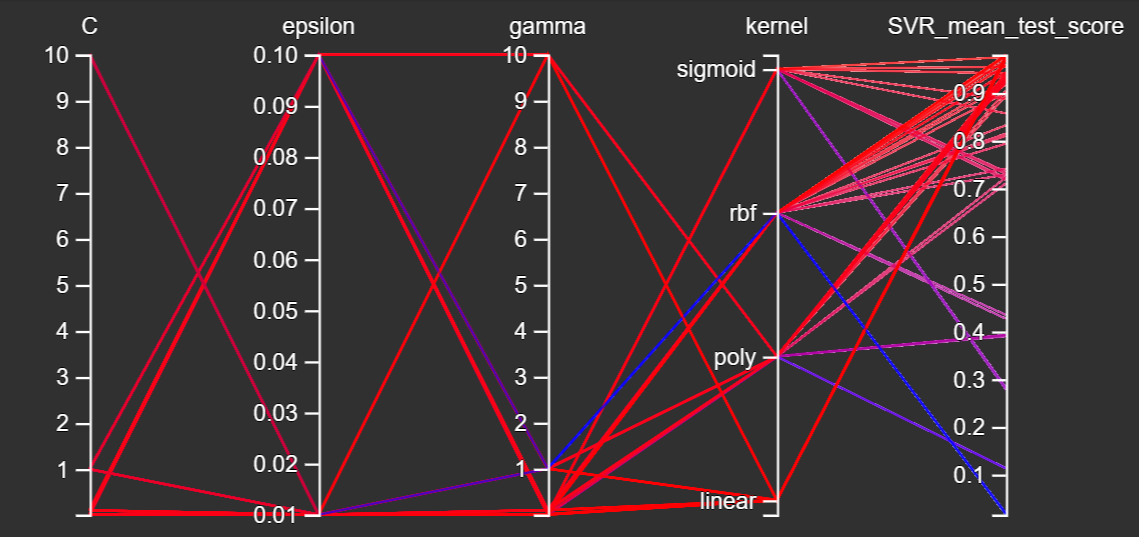
\includegraphics[width=.9\textwidth]{hpSVR.png}
\end{figure}
\subsection{KNN}
KNN è un algoritmo di ML supervisionato che permette di effettuare una regressione sui dati trovando il target predetto da un interpolazione locale dei target associati ai k piu vicini.
Abbiamo effettuato il tuning di parametri:
\begin{lstlisting}[language=Python]
    self.params = {
        'n_neighbors': [3, 5, 7, 13, 17, 25],
        'weights': ['uniform', 'distance'],
        'algorithm': ['ball_tree', 'kd_tree', 'brute'],
        'leaf_size': [10, 30, 50, 80, 100],
    }
\end{lstlisting}
Con i seguenti risultati:
\begin{table}[H]
    \centering
    \begin{tabular}{|c|c|c|}
    \hline
    \textbf{Parametri} & \textbf{senza PCA} & \textbf{PCA} \\ \hline
    \textbf{algorithm}& ball\_tree & ball\_tree\\
    \textbf{leaf\_size}& 10 &  10 \\
    \textbf{n\_neighbors}& 13 & 13\\
    \textbf{weights}& 'distance' &  'distance'\\
    \hline
\end{tabular}
\end{table}
Come per i modelli precedenti riportiamo il grafico dell'andamento dei parametri e del Mean Test Score:
\begin{figure}[H]
    \centering
    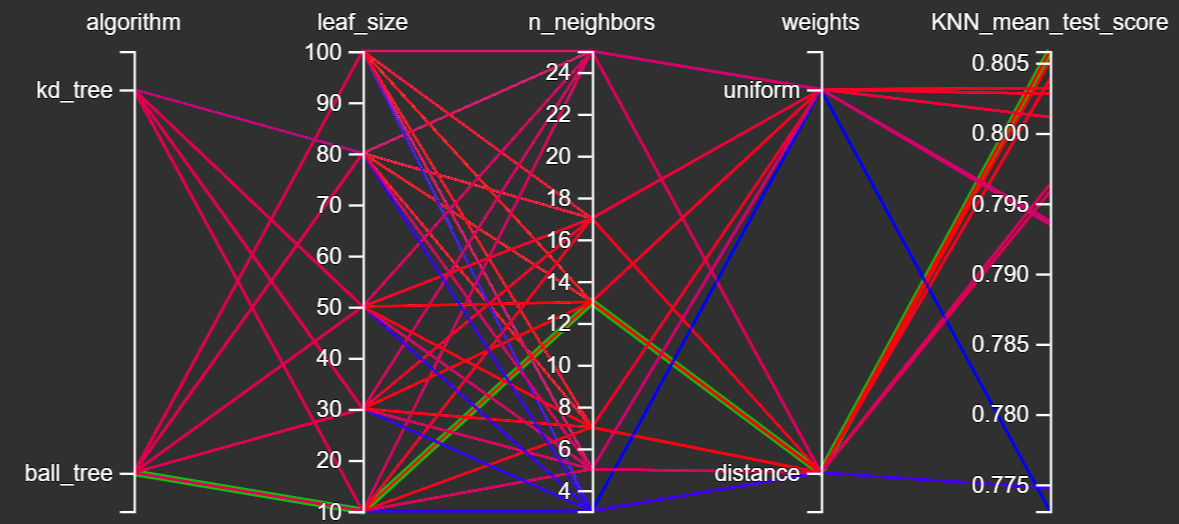
\includegraphics[width=.9\textwidth]{hpKNN.png}
\end{figure}

\subsection{Tecniche di ML Supervisionate con Reti Neurali}
Mostriamo di seguito la nostra Implementazione della Rete Neurale Feed Forward, che abbiamo utilizzato per effettuare la regressione dei dati.
Abbiamo utilizzato il framework Pytorch per la creazione della rete neurale, che ci ha permesso di utilizzare la GPU per l'addestramento della rete.

\begin{lstlisting}[language=python]
    # Define the neural network architecture
    self.model = nn.Sequential(
        nn.Linear(X.shape[1], hidden_size1),
        nn.ReLU(),
        nn.Linear(hidden_size1, hidden_size2),
        nn.ReLU(),
        nn.Linear(hidden_size2, 1)
    )

    self.criterion = nn.MSELoss()
    self.optimizer = optim.Adam(self.model.parameters(), lr=lr)

\end{lstlisting}

Abbiamo effettuato il tuning degli iperparametri della rete neurale utilizzando itertools.product, che ci ha permesso di effettuare il tuning di tutti i parametri in maniera semplice e veloce.
I parametri che abbiamo utilizzato sono:
\begin{lstlisting}[language=python]
    self.params = {
        batchsize = [128,256,512,1024]	
        hidden_size1 = [64,128,256]
        hidden_size2 = [64,128,256]
        lr = [0.0001,0.001,0.01]
        num_epochs = [200,400,600]
    }
\end{lstlisting}
I risultati ottenuti sono:
\begin{table}[H]
    \centering
    \begin{tabular}{|c|c|c|}
    \hline
    \textbf{Parametri} & \textbf{senza PCA} & \textbf{PCA} \\ \hline
    \textbf{batchsize}& 1024 & 256\\
    \textbf{hidden\_size1}& 64 &  128 \\
    \textbf{hidden\_size2}& 256 & 256\\
    \textbf{lr}& 0.01 &  0.001\\
    \textbf{num\_epochs}& 400 & 600\\
    \hline
\end{tabular}
\end{table}

Visualizziamo il grafico dell'andamento dei parametri e del Mean Test Score:
\begin{figure}[H]-
    \centering
    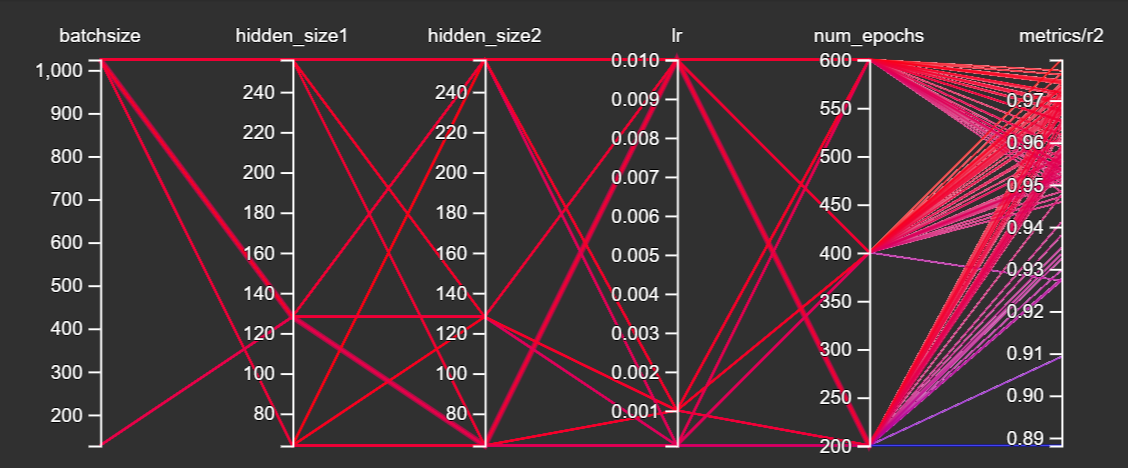
\includegraphics[width=.9\textwidth]{hpNN.png}
    \caption{Andamento dei parametri e del Mean Test Score per la Rete Neurale (senza PCA)}
\end{figure}

\section{Tabular Data}
Per quanto riguarda i Tabular Data abbiamo fatto il tuning dei seguenti iperparametri(sempre utilizzando itertools.product):
\begin{lstlisting}[language=Python]
    batchsize = [512,1024,2048]
    width = [8,16,32]
    steps = [3,5,7]
    learning_rate = [2e-2,1e-2,5e-3]    
    max_epochs = [70,120,150,210]
\end{lstlisting}
dove $width$ corrisponde a $n\_d$ e $n\_a$ dove $n\_d$ è la Larghezza del livello di previsione delle decisioni($n_a$ nella documentazione viene consigliato sia uguale a $n_d$, per questo motivo utilizziamo un singolo valore).
Viene fatto uso di Early Stopping per evitare l'overfitting.
I risultati ottenuti sono:
\begin{table}[h]
    \centering
    \begin{tabular}{|c|c|c|}
    \hline
    \textbf{Parametri} & \textbf{senza PCA} & \textbf{PCA} \\ \hline
    \textbf{batchsize}& 512 & 512 \\
    \textbf{width}& 32 & 32\\
    \textbf{steps}& 7 & 5\\
    \textbf{learning\_rate}&  0.02 & 0.02 \\
    \textbf{max\_epochs}& 70& 150 \\
    \hline
    \end{tabular}
\end{table}

Con un andamento degli iperparametri e del Mean Test Score come segue:
\begin{figure}[H]
    \centering
    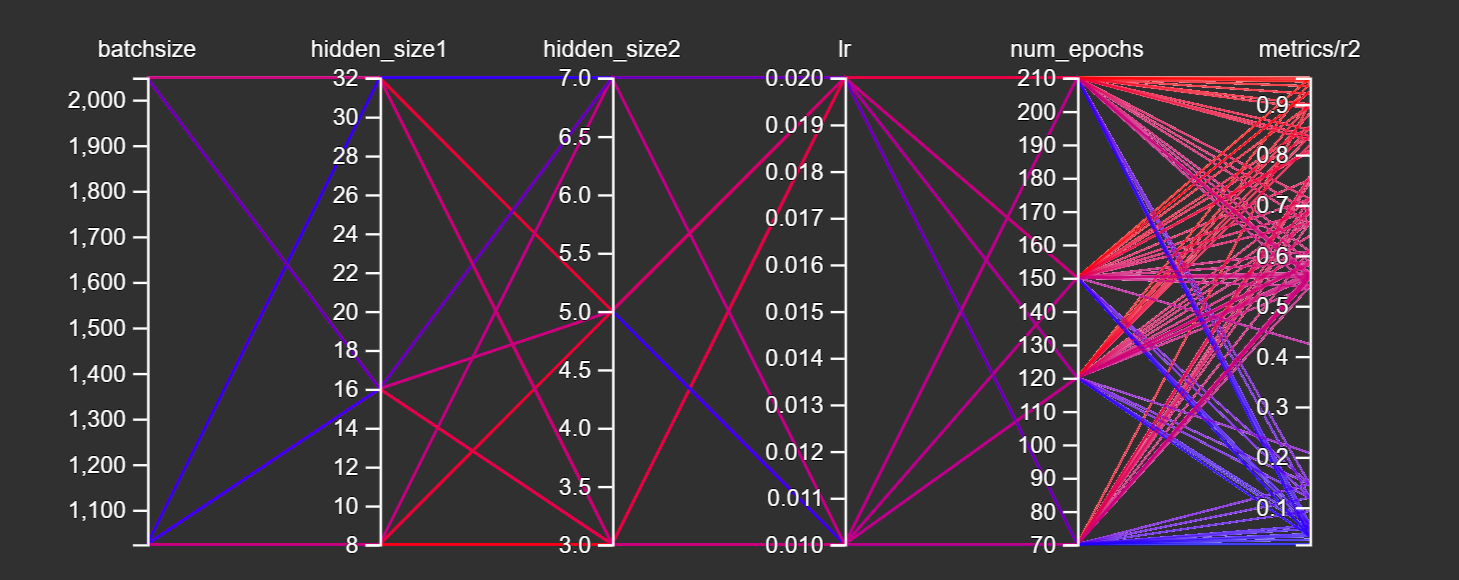
\includegraphics[width=.9\textwidth]{hpTabular.png}
    \caption{Andamento dei parametri e del Mean Test Score per i Tabular Data (senza PCA)}
\end{figure}
\end{document}